\documentclass[]{book}
\usepackage{lmodern}
\usepackage{amssymb,amsmath}
\usepackage{ifxetex,ifluatex}
\usepackage{fixltx2e} % provides \textsubscript
\ifnum 0\ifxetex 1\fi\ifluatex 1\fi=0 % if pdftex
  \usepackage[T1]{fontenc}
  \usepackage[utf8]{inputenc}
\else % if luatex or xelatex
  \ifxetex
    \usepackage{mathspec}
  \else
    \usepackage{fontspec}
  \fi
  \defaultfontfeatures{Ligatures=TeX,Scale=MatchLowercase}
\fi
% use upquote if available, for straight quotes in verbatim environments
\IfFileExists{upquote.sty}{\usepackage{upquote}}{}
% use microtype if available
\IfFileExists{microtype.sty}{%
\usepackage{microtype}
\UseMicrotypeSet[protrusion]{basicmath} % disable protrusion for tt fonts
}{}
\usepackage{hyperref}
\hypersetup{unicode=true,
            pdftitle={R},
            pdfauthor={Bill Last Updated:},
            pdfborder={0 0 0},
            breaklinks=true}
\urlstyle{same}  % don't use monospace font for urls
\usepackage{natbib}
\bibliographystyle{apalike}
\usepackage{color}
\usepackage{fancyvrb}
\newcommand{\VerbBar}{|}
\newcommand{\VERB}{\Verb[commandchars=\\\{\}]}
\DefineVerbatimEnvironment{Highlighting}{Verbatim}{commandchars=\\\{\}}
% Add ',fontsize=\small' for more characters per line
\usepackage{framed}
\definecolor{shadecolor}{RGB}{248,248,248}
\newenvironment{Shaded}{\begin{snugshade}}{\end{snugshade}}
\newcommand{\AlertTok}[1]{\textcolor[rgb]{0.94,0.16,0.16}{#1}}
\newcommand{\AnnotationTok}[1]{\textcolor[rgb]{0.56,0.35,0.01}{\textbf{\textit{#1}}}}
\newcommand{\AttributeTok}[1]{\textcolor[rgb]{0.77,0.63,0.00}{#1}}
\newcommand{\BaseNTok}[1]{\textcolor[rgb]{0.00,0.00,0.81}{#1}}
\newcommand{\BuiltInTok}[1]{#1}
\newcommand{\CharTok}[1]{\textcolor[rgb]{0.31,0.60,0.02}{#1}}
\newcommand{\CommentTok}[1]{\textcolor[rgb]{0.56,0.35,0.01}{\textit{#1}}}
\newcommand{\CommentVarTok}[1]{\textcolor[rgb]{0.56,0.35,0.01}{\textbf{\textit{#1}}}}
\newcommand{\ConstantTok}[1]{\textcolor[rgb]{0.00,0.00,0.00}{#1}}
\newcommand{\ControlFlowTok}[1]{\textcolor[rgb]{0.13,0.29,0.53}{\textbf{#1}}}
\newcommand{\DataTypeTok}[1]{\textcolor[rgb]{0.13,0.29,0.53}{#1}}
\newcommand{\DecValTok}[1]{\textcolor[rgb]{0.00,0.00,0.81}{#1}}
\newcommand{\DocumentationTok}[1]{\textcolor[rgb]{0.56,0.35,0.01}{\textbf{\textit{#1}}}}
\newcommand{\ErrorTok}[1]{\textcolor[rgb]{0.64,0.00,0.00}{\textbf{#1}}}
\newcommand{\ExtensionTok}[1]{#1}
\newcommand{\FloatTok}[1]{\textcolor[rgb]{0.00,0.00,0.81}{#1}}
\newcommand{\FunctionTok}[1]{\textcolor[rgb]{0.00,0.00,0.00}{#1}}
\newcommand{\ImportTok}[1]{#1}
\newcommand{\InformationTok}[1]{\textcolor[rgb]{0.56,0.35,0.01}{\textbf{\textit{#1}}}}
\newcommand{\KeywordTok}[1]{\textcolor[rgb]{0.13,0.29,0.53}{\textbf{#1}}}
\newcommand{\NormalTok}[1]{#1}
\newcommand{\OperatorTok}[1]{\textcolor[rgb]{0.81,0.36,0.00}{\textbf{#1}}}
\newcommand{\OtherTok}[1]{\textcolor[rgb]{0.56,0.35,0.01}{#1}}
\newcommand{\PreprocessorTok}[1]{\textcolor[rgb]{0.56,0.35,0.01}{\textit{#1}}}
\newcommand{\RegionMarkerTok}[1]{#1}
\newcommand{\SpecialCharTok}[1]{\textcolor[rgb]{0.00,0.00,0.00}{#1}}
\newcommand{\SpecialStringTok}[1]{\textcolor[rgb]{0.31,0.60,0.02}{#1}}
\newcommand{\StringTok}[1]{\textcolor[rgb]{0.31,0.60,0.02}{#1}}
\newcommand{\VariableTok}[1]{\textcolor[rgb]{0.00,0.00,0.00}{#1}}
\newcommand{\VerbatimStringTok}[1]{\textcolor[rgb]{0.31,0.60,0.02}{#1}}
\newcommand{\WarningTok}[1]{\textcolor[rgb]{0.56,0.35,0.01}{\textbf{\textit{#1}}}}
\usepackage{longtable,booktabs}
\usepackage{graphicx,grffile}
\makeatletter
\def\maxwidth{\ifdim\Gin@nat@width>\linewidth\linewidth\else\Gin@nat@width\fi}
\def\maxheight{\ifdim\Gin@nat@height>\textheight\textheight\else\Gin@nat@height\fi}
\makeatother
% Scale images if necessary, so that they will not overflow the page
% margins by default, and it is still possible to overwrite the defaults
% using explicit options in \includegraphics[width, height, ...]{}
\setkeys{Gin}{width=\maxwidth,height=\maxheight,keepaspectratio}
\IfFileExists{parskip.sty}{%
\usepackage{parskip}
}{% else
\setlength{\parindent}{0pt}
\setlength{\parskip}{6pt plus 2pt minus 1pt}
}
\setlength{\emergencystretch}{3em}  % prevent overfull lines
\providecommand{\tightlist}{%
  \setlength{\itemsep}{0pt}\setlength{\parskip}{0pt}}
\setcounter{secnumdepth}{5}
% Redefines (sub)paragraphs to behave more like sections
\ifx\paragraph\undefined\else
\let\oldparagraph\paragraph
\renewcommand{\paragraph}[1]{\oldparagraph{#1}\mbox{}}
\fi
\ifx\subparagraph\undefined\else
\let\oldsubparagraph\subparagraph
\renewcommand{\subparagraph}[1]{\oldsubparagraph{#1}\mbox{}}
\fi

%%% Use protect on footnotes to avoid problems with footnotes in titles
\let\rmarkdownfootnote\footnote%
\def\footnote{\protect\rmarkdownfootnote}

%%% Change title format to be more compact
\usepackage{titling}

% Create subtitle command for use in maketitle
\providecommand{\subtitle}[1]{
  \posttitle{
    \begin{center}\large#1\end{center}
    }
}

\setlength{\droptitle}{-2em}

  \title{R}
    \pretitle{\vspace{\droptitle}\centering\huge}
  \posttitle{\par}
    \author{Bill Last Updated:}
    \preauthor{\centering\large\emph}
  \postauthor{\par}
      \predate{\centering\large\emph}
  \postdate{\par}
    \date{10 April, 2020}

\usepackage{booktabs}
\usepackage{amsthm}
\makeatletter
\def\thm@space@setup{%
  \thm@preskip=8pt plus 2pt minus 4pt
  \thm@postskip=\thm@preskip
}
\makeatother

\begin{document}
\maketitle

{
\setcounter{tocdepth}{1}
\tableofcontents
}
\hypertarget{my-section}{%
\chapter*{Preface: Motivation}\label{my-section}}
\addcontentsline{toc}{chapter}{Preface: Motivation}

All the notes I have done here are about R. While I have tried my best, probably there are still some typos and errors. Please feel free to let me know in case you find one. Thank you!

\hypertarget{apply-lapply-sapply}{%
\chapter{apply, lapply, sapply}\label{apply-lapply-sapply}}

\hypertarget{apply}{%
\section{apply}\label{apply}}

\begin{Shaded}
\begin{Highlighting}[]
\NormalTok{m_trying <-}\StringTok{ }\KeywordTok{matrix}\NormalTok{(C<-(}\DecValTok{1}\OperatorTok{:}\DecValTok{10}\NormalTok{),}\DataTypeTok{nrow=}\DecValTok{2}\NormalTok{, }\DataTypeTok{ncol=}\DecValTok{5}\NormalTok{)}
\NormalTok{m_trying}
\end{Highlighting}
\end{Shaded}

\begin{verbatim}
##      [,1] [,2] [,3] [,4] [,5]
## [1,]    1    3    5    7    9
## [2,]    2    4    6    8   10
\end{verbatim}

\begin{Shaded}
\begin{Highlighting}[]
\CommentTok{## Operating on the columns}
\KeywordTok{apply}\NormalTok{(m_trying, }\DecValTok{2}\NormalTok{, sum)}
\end{Highlighting}
\end{Shaded}

\begin{verbatim}
## [1]  3  7 11 15 19
\end{verbatim}

\begin{Shaded}
\begin{Highlighting}[]
\CommentTok{## Operating on the rows}
\KeywordTok{apply}\NormalTok{(m_trying, }\DecValTok{1}\NormalTok{, sum)}
\end{Highlighting}
\end{Shaded}

\begin{verbatim}
## [1] 25 30
\end{verbatim}

\hypertarget{lapply}{%
\section{lapply}\label{lapply}}

``lapply returns a list of the same length as X, each element of which is the result of applying FUN to the corresponding element of X.''

lapply operates on lists. Thus, as we can see below, even if m\_trying is not a list, each cell becomes a list.

\begin{Shaded}
\begin{Highlighting}[]
\NormalTok{results1<-}\KeywordTok{lapply}\NormalTok{(m_trying,sum)}
\KeywordTok{str}\NormalTok{(results1)}
\end{Highlighting}
\end{Shaded}

\begin{verbatim}
## List of 10
##  $ : int 1
##  $ : int 2
##  $ : int 3
##  $ : int 4
##  $ : int 5
##  $ : int 6
##  $ : int 7
##  $ : int 8
##  $ : int 9
##  $ : int 10
\end{verbatim}

\begin{Shaded}
\begin{Highlighting}[]
\KeywordTok{is.list}\NormalTok{(results1)}
\end{Highlighting}
\end{Shaded}

\begin{verbatim}
## [1] TRUE
\end{verbatim}

\hypertarget{sapply}{%
\section{sapply}\label{sapply}}

``sapply() function takes list, vector or data frame as input and gives output in vector or matrix.''

\begin{Shaded}
\begin{Highlighting}[]
\NormalTok{results2<-}\KeywordTok{sapply}\NormalTok{(m_trying, sum)}
\KeywordTok{str}\NormalTok{(results2)}
\end{Highlighting}
\end{Shaded}

\begin{verbatim}
##  int [1:10] 1 2 3 4 5 6 7 8 9 10
\end{verbatim}

\begin{Shaded}
\begin{Highlighting}[]
\KeywordTok{is.list}\NormalTok{(results2)}
\end{Highlighting}
\end{Shaded}

\begin{verbatim}
## [1] FALSE
\end{verbatim}

\begin{Shaded}
\begin{Highlighting}[]
\KeywordTok{is.matrix}\NormalTok{(results2)}
\end{Highlighting}
\end{Shaded}

\begin{verbatim}
## [1] FALSE
\end{verbatim}

\begin{Shaded}
\begin{Highlighting}[]
\KeywordTok{is.data.frame}\NormalTok{(results2)}
\end{Highlighting}
\end{Shaded}

\begin{verbatim}
## [1] FALSE
\end{verbatim}

\begin{Shaded}
\begin{Highlighting}[]
\KeywordTok{is.vector}\NormalTok{(results2)}
\end{Highlighting}
\end{Shaded}

\begin{verbatim}
## [1] TRUE
\end{verbatim}

\hypertarget{c}{%
\chapter{C}\label{c}}

\begin{Shaded}
\begin{Highlighting}[]
\NormalTok{mydata1<-}\KeywordTok{matrix}\NormalTok{(}\KeywordTok{runif}\NormalTok{(}\DecValTok{4}\OperatorTok{*}\DecValTok{2}\NormalTok{),}\DecValTok{4}\NormalTok{,}\DecValTok{2}\NormalTok{)}
\NormalTok{mydata1}
\end{Highlighting}
\end{Shaded}

\begin{verbatim}
##           [,1]      [,2]
## [1,] 0.1969175 0.2054529
## [2,] 0.6757720 0.9610585
## [3,] 0.5566467 0.3911608
## [4,] 0.7862333 0.4072791
\end{verbatim}

\begin{Shaded}
\begin{Highlighting}[]
\KeywordTok{str}\NormalTok{(mydata1)}
\end{Highlighting}
\end{Shaded}

\begin{verbatim}
##  num [1:4, 1:2] 0.197 0.676 0.557 0.786 0.205 ...
\end{verbatim}

\begin{Shaded}
\begin{Highlighting}[]
\NormalTok{mydata2<-}\KeywordTok{c}\NormalTok{(mydata1)}
\NormalTok{mydata2}
\end{Highlighting}
\end{Shaded}

\begin{verbatim}
## [1] 0.1969175 0.6757720 0.5566467 0.7862333 0.2054529 0.9610585 0.3911608
## [8] 0.4072791
\end{verbatim}

\begin{Shaded}
\begin{Highlighting}[]
\KeywordTok{str}\NormalTok{(mydata2)}
\end{Highlighting}
\end{Shaded}

\begin{verbatim}
##  num [1:8] 0.197 0.676 0.557 0.786 0.205 ...
\end{verbatim}

\hypertarget{glm-and-glim}{%
\chapter{GLM and GLiM}\label{glm-and-glim}}

\begin{Shaded}
\begin{Highlighting}[]
\NormalTok{data2<-}\KeywordTok{seq}\NormalTok{(}\OperatorTok{-}\DecValTok{5}\NormalTok{,}\DecValTok{5}\NormalTok{,}\DecValTok{1}\NormalTok{)}
\KeywordTok{plot}\NormalTok{(data2,}\KeywordTok{pnorm}\NormalTok{(data2),}\DataTypeTok{type =} \StringTok{"b"}\NormalTok{)}
\end{Highlighting}
\end{Shaded}

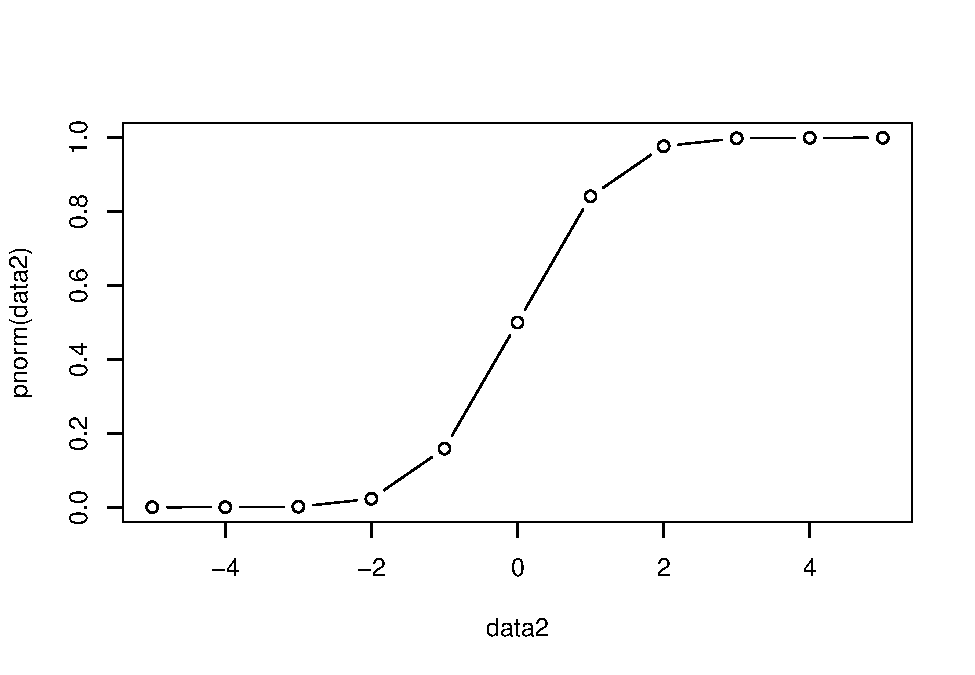
\includegraphics{bookdown-demo_files/figure-latex/unnamed-chunk-5-1.pdf}

\begin{Shaded}
\begin{Highlighting}[]
\NormalTok{b_}\DecValTok{1}\NormalTok{<-}\DecValTok{2}

\NormalTok{x<-}\KeywordTok{rnorm}\NormalTok{(}\DecValTok{1000}\NormalTok{)}
\NormalTok{y=b_}\DecValTok{1}\OperatorTok{*}\NormalTok{x}\OperatorTok{+}\KeywordTok{rnorm}\NormalTok{(}\DecValTok{1000}\NormalTok{)}
\KeywordTok{plot}\NormalTok{(x,y)}
\end{Highlighting}
\end{Shaded}

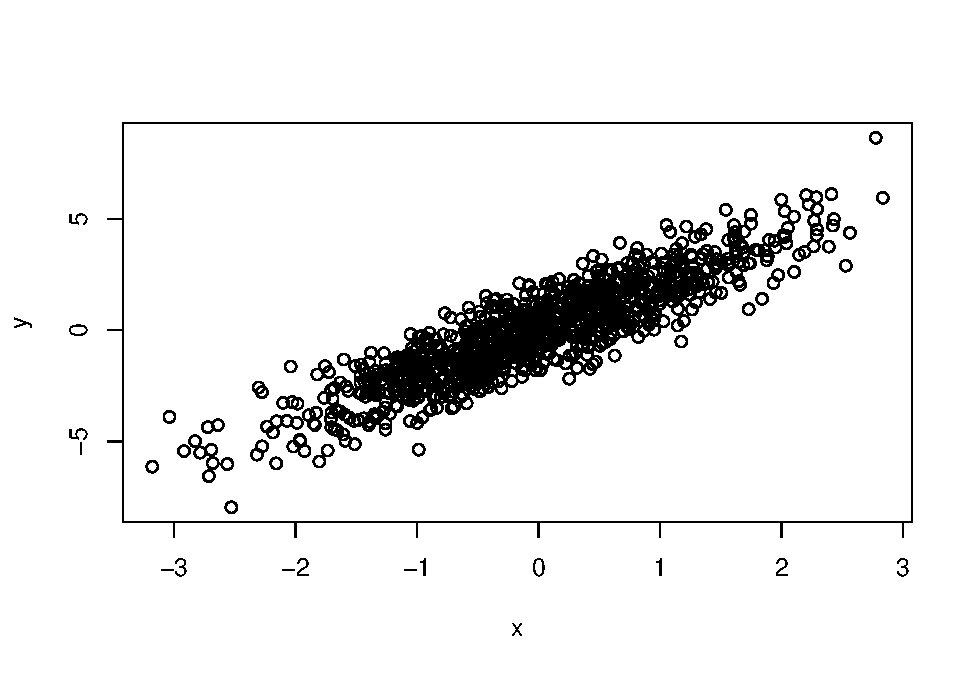
\includegraphics{bookdown-demo_files/figure-latex/unnamed-chunk-5-2.pdf}

\begin{Shaded}
\begin{Highlighting}[]
\NormalTok{data_}\DecValTok{1}\NormalTok{<-}\KeywordTok{as.data.frame}\NormalTok{(}\KeywordTok{cbind}\NormalTok{(y,x)) }

\KeywordTok{library}\NormalTok{(ggplot2)}
\KeywordTok{ggplot}\NormalTok{(data_}\DecValTok{1}\NormalTok{,}\KeywordTok{aes}\NormalTok{(x, y)) }\OperatorTok{+}
\StringTok{  }\KeywordTok{geom_point}\NormalTok{() }\OperatorTok{+}
\StringTok{  }\KeywordTok{geom_smooth}\NormalTok{(}\DataTypeTok{method =} \StringTok{"lm"}\NormalTok{)}\OperatorTok{+}\KeywordTok{theme_classic}\NormalTok{()}
\end{Highlighting}
\end{Shaded}

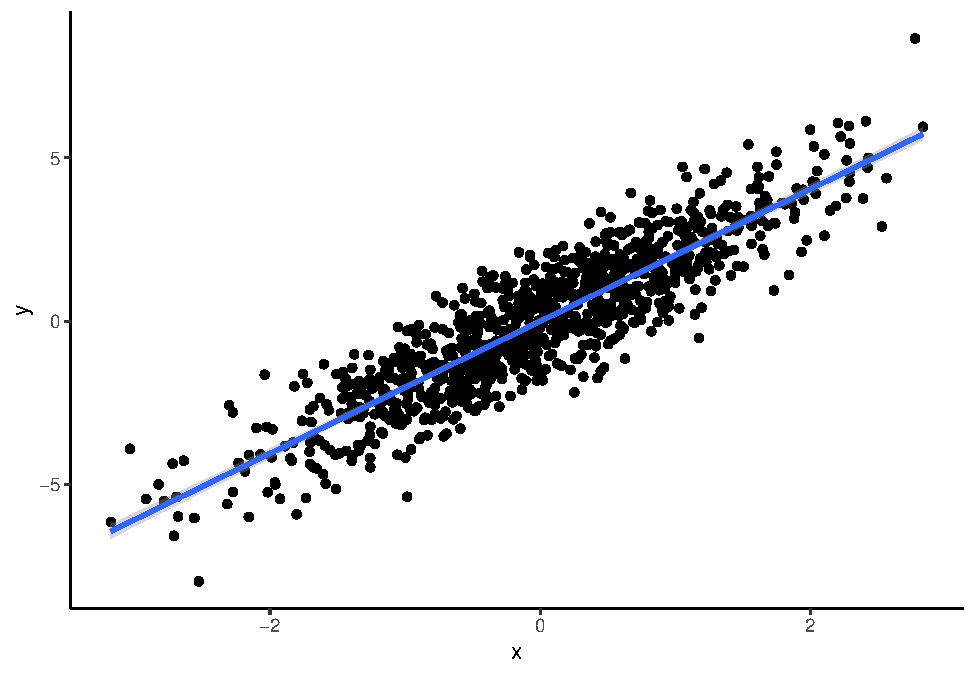
\includegraphics{bookdown-demo_files/figure-latex/unnamed-chunk-5-3.pdf}

\begin{Shaded}
\begin{Highlighting}[]
\NormalTok{x<-}\KeywordTok{rnorm}\NormalTok{(}\DecValTok{1000}\NormalTok{)}
\NormalTok{y=b_}\DecValTok{1}\OperatorTok{*}\NormalTok{x}\OperatorTok{+}\KeywordTok{rnorm}\NormalTok{(}\DecValTok{1000}\NormalTok{)}
\NormalTok{mu=}\KeywordTok{exp}\NormalTok{(y)}\OperatorTok{/}\NormalTok{(}\DecValTok{1}\OperatorTok{+}\KeywordTok{exp}\NormalTok{(y))}


\NormalTok{u<-}\KeywordTok{runif}\NormalTok{(}\DecValTok{1000}\NormalTok{)}
\NormalTok{binary_Y<-}\KeywordTok{ifelse}\NormalTok{(mu}\OperatorTok{>}\NormalTok{u,}\DecValTok{1}\NormalTok{,}\DecValTok{0}\NormalTok{)}
\NormalTok{data_}\DecValTok{2}\NormalTok{<-}\KeywordTok{as.data.frame}\NormalTok{(}\KeywordTok{cbind}\NormalTok{(binary_Y,x)) }

\KeywordTok{library}\NormalTok{(ggplot2)}
\KeywordTok{ggplot}\NormalTok{(data_}\DecValTok{2}\NormalTok{,}\KeywordTok{aes}\NormalTok{(x, binary_Y)) }\OperatorTok{+}
\StringTok{  }\KeywordTok{geom_point}\NormalTok{() }\OperatorTok{+}
\StringTok{  }\KeywordTok{geom_smooth}\NormalTok{(}\DataTypeTok{method =} \StringTok{"glm"}\NormalTok{, }\DataTypeTok{method.args =} \KeywordTok{list}\NormalTok{(}\DataTypeTok{family =} \StringTok{"binomial"}\NormalTok{), }
              \DataTypeTok{se =} \OtherTok{FALSE}\NormalTok{)}\OperatorTok{+}\KeywordTok{theme_classic}\NormalTok{()}
\end{Highlighting}
\end{Shaded}

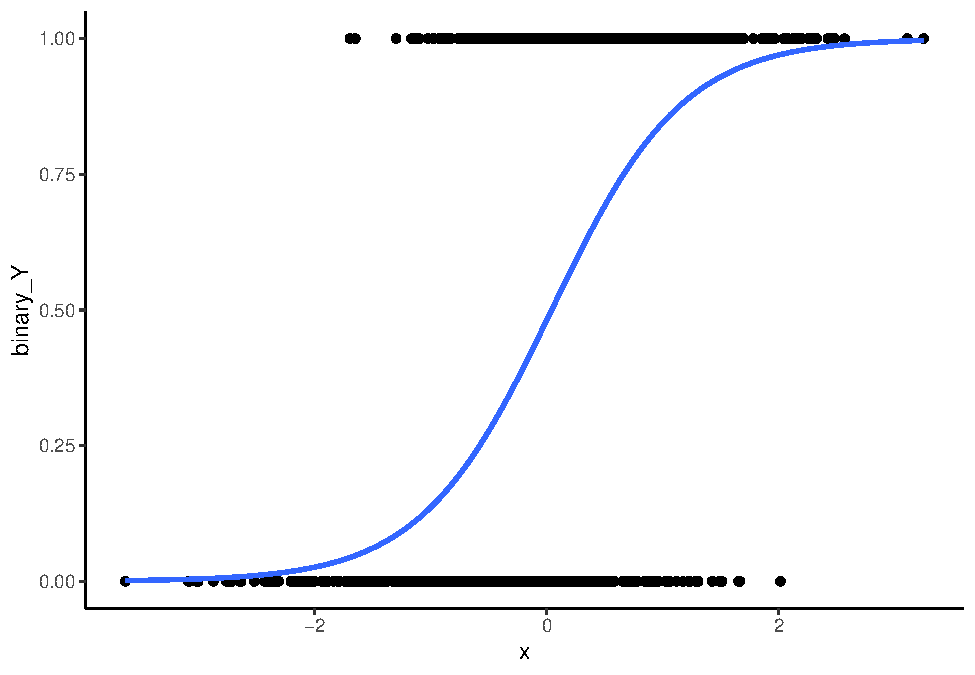
\includegraphics{bookdown-demo_files/figure-latex/unnamed-chunk-5-4.pdf}

\hypertarget{tidyverse}{%
\chapter{Tidyverse}\label{tidyverse}}

\hypertarget{slice}{%
\section{Slice}\label{slice}}

\url{https://dplyr.tidyverse.org/reference/slice.html}

\begin{Shaded}
\begin{Highlighting}[]
\NormalTok{mtcars}
\end{Highlighting}
\end{Shaded}

\begin{verbatim}
##                      mpg cyl  disp  hp drat    wt  qsec vs am gear carb
## Mazda RX4           21.0   6 160.0 110 3.90 2.620 16.46  0  1    4    4
## Mazda RX4 Wag       21.0   6 160.0 110 3.90 2.875 17.02  0  1    4    4
## Datsun 710          22.8   4 108.0  93 3.85 2.320 18.61  1  1    4    1
## Hornet 4 Drive      21.4   6 258.0 110 3.08 3.215 19.44  1  0    3    1
## Hornet Sportabout   18.7   8 360.0 175 3.15 3.440 17.02  0  0    3    2
## Valiant             18.1   6 225.0 105 2.76 3.460 20.22  1  0    3    1
## Duster 360          14.3   8 360.0 245 3.21 3.570 15.84  0  0    3    4
## Merc 240D           24.4   4 146.7  62 3.69 3.190 20.00  1  0    4    2
## Merc 230            22.8   4 140.8  95 3.92 3.150 22.90  1  0    4    2
## Merc 280            19.2   6 167.6 123 3.92 3.440 18.30  1  0    4    4
## Merc 280C           17.8   6 167.6 123 3.92 3.440 18.90  1  0    4    4
## Merc 450SE          16.4   8 275.8 180 3.07 4.070 17.40  0  0    3    3
## Merc 450SL          17.3   8 275.8 180 3.07 3.730 17.60  0  0    3    3
## Merc 450SLC         15.2   8 275.8 180 3.07 3.780 18.00  0  0    3    3
## Cadillac Fleetwood  10.4   8 472.0 205 2.93 5.250 17.98  0  0    3    4
## Lincoln Continental 10.4   8 460.0 215 3.00 5.424 17.82  0  0    3    4
## Chrysler Imperial   14.7   8 440.0 230 3.23 5.345 17.42  0  0    3    4
## Fiat 128            32.4   4  78.7  66 4.08 2.200 19.47  1  1    4    1
## Honda Civic         30.4   4  75.7  52 4.93 1.615 18.52  1  1    4    2
## Toyota Corolla      33.9   4  71.1  65 4.22 1.835 19.90  1  1    4    1
## Toyota Corona       21.5   4 120.1  97 3.70 2.465 20.01  1  0    3    1
## Dodge Challenger    15.5   8 318.0 150 2.76 3.520 16.87  0  0    3    2
## AMC Javelin         15.2   8 304.0 150 3.15 3.435 17.30  0  0    3    2
## Camaro Z28          13.3   8 350.0 245 3.73 3.840 15.41  0  0    3    4
## Pontiac Firebird    19.2   8 400.0 175 3.08 3.845 17.05  0  0    3    2
## Fiat X1-9           27.3   4  79.0  66 4.08 1.935 18.90  1  1    4    1
## Porsche 914-2       26.0   4 120.3  91 4.43 2.140 16.70  0  1    5    2
## Lotus Europa        30.4   4  95.1 113 3.77 1.513 16.90  1  1    5    2
## Ford Pantera L      15.8   8 351.0 264 4.22 3.170 14.50  0  1    5    4
## Ferrari Dino        19.7   6 145.0 175 3.62 2.770 15.50  0  1    5    6
## Maserati Bora       15.0   8 301.0 335 3.54 3.570 14.60  0  1    5    8
## Volvo 142E          21.4   4 121.0 109 4.11 2.780 18.60  1  1    4    2
\end{verbatim}

\begin{Shaded}
\begin{Highlighting}[]
\KeywordTok{library}\NormalTok{(tidyverse)}
\KeywordTok{slice}\NormalTok{(mtcars,1L)}
\end{Highlighting}
\end{Shaded}

\begin{verbatim}
##   mpg cyl disp  hp drat   wt  qsec vs am gear carb
## 1  21   6  160 110  3.9 2.62 16.46  0  1    4    4
\end{verbatim}

\begin{Shaded}
\begin{Highlighting}[]
\KeywordTok{slice}\NormalTok{(mtcars,}\KeywordTok{n}\NormalTok{())}
\end{Highlighting}
\end{Shaded}

\begin{verbatim}
##    mpg cyl disp  hp drat   wt qsec vs am gear carb
## 1 21.4   4  121 109 4.11 2.78 18.6  1  1    4    2
\end{verbatim}

Group\_by just group row with same values (w.r.t a certain column) together. It does not reduce row number.

\hypertarget{group_by}{%
\section{Group\_by}\label{group_by}}

\begin{Shaded}
\begin{Highlighting}[]
\NormalTok{by_cyl<-}\KeywordTok{group_by}\NormalTok{(mtcars,cyl)}

\NormalTok{by_cyl}
\end{Highlighting}
\end{Shaded}

\begin{verbatim}
## # A tibble: 32 x 11
## # Groups:   cyl [3]
##      mpg   cyl  disp    hp  drat    wt  qsec    vs    am  gear  carb
##  * <dbl> <dbl> <dbl> <dbl> <dbl> <dbl> <dbl> <dbl> <dbl> <dbl> <dbl>
##  1  21       6  160    110  3.9   2.62  16.5     0     1     4     4
##  2  21       6  160    110  3.9   2.88  17.0     0     1     4     4
##  3  22.8     4  108     93  3.85  2.32  18.6     1     1     4     1
##  4  21.4     6  258    110  3.08  3.22  19.4     1     0     3     1
##  5  18.7     8  360    175  3.15  3.44  17.0     0     0     3     2
##  6  18.1     6  225    105  2.76  3.46  20.2     1     0     3     1
##  7  14.3     8  360    245  3.21  3.57  15.8     0     0     3     4
##  8  24.4     4  147.    62  3.69  3.19  20       1     0     4     2
##  9  22.8     4  141.    95  3.92  3.15  22.9     1     0     4     2
## 10  19.2     6  168.   123  3.92  3.44  18.3     1     0     4     4
## # ... with 22 more rows
\end{verbatim}

\begin{Shaded}
\begin{Highlighting}[]
\KeywordTok{nrow}\NormalTok{(mtcars)}
\end{Highlighting}
\end{Shaded}

\begin{verbatim}
## [1] 32
\end{verbatim}

\begin{Shaded}
\begin{Highlighting}[]
\KeywordTok{nrow}\NormalTok{(by_cyl)}
\end{Highlighting}
\end{Shaded}

\begin{verbatim}
## [1] 32
\end{verbatim}

\hypertarget{filter}{%
\section{Filter}\label{filter}}

You can also use \textbf{filter} to do the same job as \textbf{slice} . The only difference is that you need to provide a variable name.

\begin{Shaded}
\begin{Highlighting}[]
\KeywordTok{filter}\NormalTok{(mtcars, }\KeywordTok{row_number}\NormalTok{()}\OperatorTok{==}\NormalTok{1L)}
\end{Highlighting}
\end{Shaded}

\begin{verbatim}
##   mpg cyl disp  hp drat   wt  qsec vs am gear carb
## 1  21   6  160 110  3.9 2.62 16.46  0  1    4    4
\end{verbatim}

\begin{Shaded}
\begin{Highlighting}[]
\KeywordTok{filter}\NormalTok{(mtcars, }\KeywordTok{row_number}\NormalTok{()}\OperatorTok{==}\KeywordTok{n}\NormalTok{())}
\end{Highlighting}
\end{Shaded}

\begin{verbatim}
##    mpg cyl disp  hp drat   wt qsec vs am gear carb
## 1 21.4   4  121 109 4.11 2.78 18.6  1  1    4    2
\end{verbatim}

\bibliography{book.bib,packages.bib}


\end{document}
